Once the code is created, I proceeded to the simulations.
In Xilinx Software I created a  \textit{test bench} in verilog to test my developed model. The bench test is a very useful tool that allows you to test the digital circuits developed without the need for hardware.
\\ In the test bench file I introduced a clock signal and several sequences of input signals.
 
 \captionof{listing}{wash\_fsm\_tb.v\label{wash_fsm_tb.v}}
 \vspace*{-2mm}
 \inputminted[
 breaklines=true,
 baselinestretch=1,
 bgcolor=Ivory,
 linenos=true,
 numbersep =0pt,	
 fontsize=\small,
 fontfamily= courier,
 obeytabs=true,
 tabsize=1,
 frame=topline,
 framesep=2mm,
 samepage= false
 firstnumber= auto,
 %firstline= 1,
 %lastline= 17
 ]{bash}{../wash_fsm_tb.v}
 
In the  \autoref{fig:sim} we have an overview of the simulation going through all 5 states in the state machine and their associated sinais.

Representation and colors of the signals in the simulation:
	\begin{itemize}
		\item Clock - Yellow
		\item Reset - Red
		\item Inputs(Buttons) - Blue
		\item Outputs (5 States + heat r) - Green
		\item Current state (binary) - Green
	\end{itemize}

\begin{figure}[H]
	\centering
	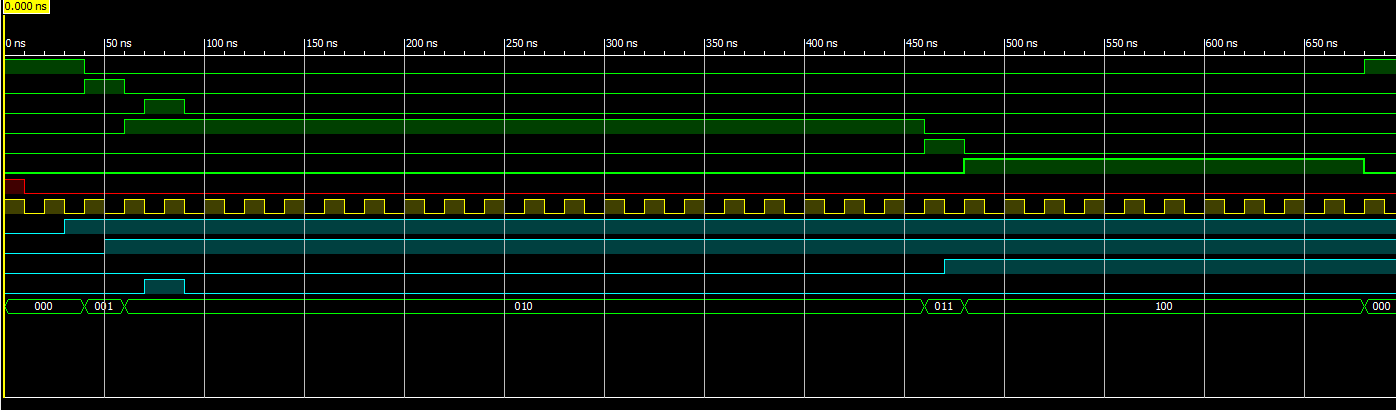
\includegraphics[width=1.1\textwidth]{img/sim}
	\caption{Overview of simulation with all existing state and signals{}}
	\label{fig:sim}
\end{figure}

The transition between the first three states is in \autoref{fig:Capture1}.

\begin{figure}[H]
	\centering
	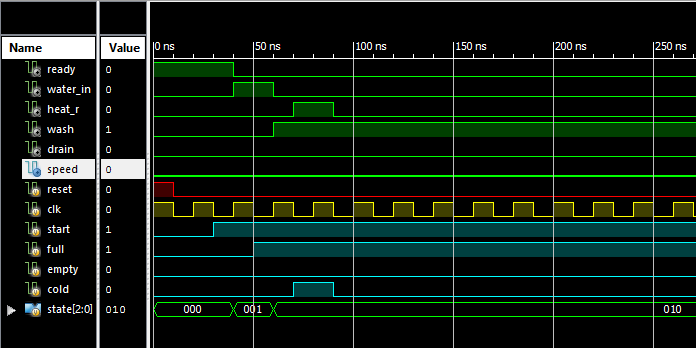
\includegraphics[width=1\textwidth]{img/Capture1}
	\caption{View of the simulation with the first 3 states}
	\label{fig:Capture1}
\end{figure}

The dwell time in the state \textit{wash} was changed from 4s to 400ns to be faster the simulation analysis as it happens in the \autoref{fig:Capture2}.

\begin{figure}[H]
	\centering
	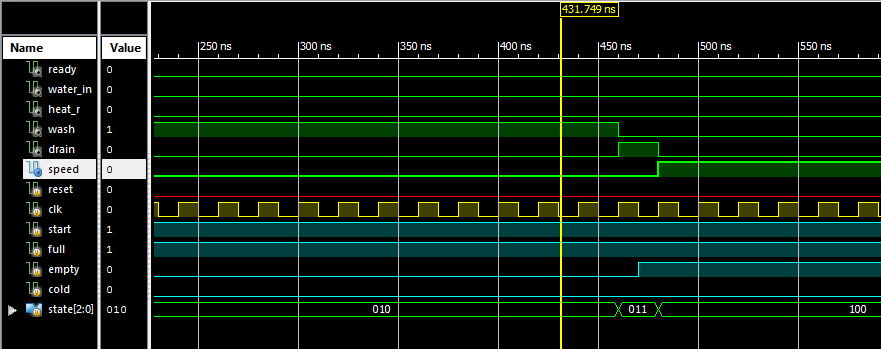
\includegraphics[width=1\textwidth]{img/Capture2}
	\caption{View of the simulation with states 2, 3 and 4}
	\label{fig:Capture2}
\end{figure}

The dwell time in the \textit{speed} state has been changed from 2s to 200ns to be faster to analyze the simulation \autoref{fig:Capture3}.

\begin{figure}[H]
	\centering
	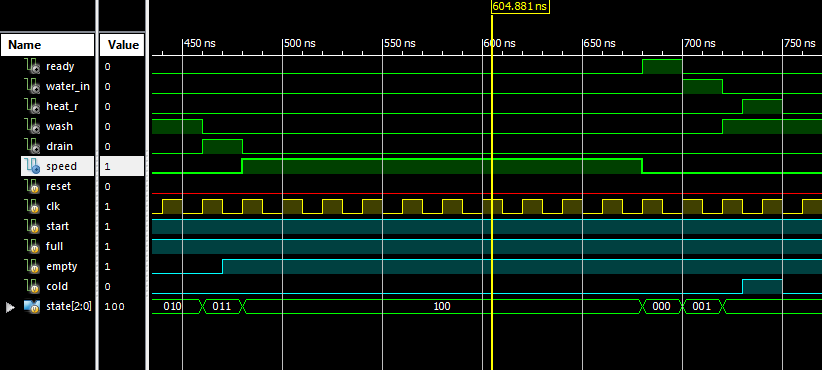
\includegraphics[width=1\textwidth]{img/Capture3}
	\caption{View of the simulation with states 2, 3, 4, 0, 1 and 2}
	\label{fig:Capture3}
\end{figure}